\documentclass{beamer}

\mode<presentation> {
	\usetheme{CambridgeUS}      % or try Darmstadt, Madrid, Warsaw, ...
	\usecolortheme{default} % or try albatross, beaver, crane, ...
	\usefonttheme{default}  % or try serif, structurebold, ...
	\setbeamertemplate{navigation symbols}{}
	\setbeamertemplate{caption}[numbered]
}

\usepackage[utf8]{inputenc}
\usepackage[T1]{fontenc}
\usepackage[french]{babel}

\usepackage{amsmath}
\usepackage{amssymb}
\usepackage{alltt}
\usepackage{graphicx}
\usepackage{subcaption}
\usepackage{tabularx}

\usepackage{makecell}

\usepackage[fixlanguage]{babelbib}
\selectbiblanguage{french}

\title[Kernalytics]{Méthodes à noyaux: théorie, implémentation et utilisation}
\author[VK]{Vincent KUBICKI - InriaTech}
\institute[Inria]{Inria Lille - Nord Europe}
\date{22 Juin 2018}

\begin{document}

\begin{frame}[plain]
	\titlepage
\end{frame}

\section{Introduction}

% Faire une petite biblio par exemple kernel methods vs neural networks

\begin{frame}{Généralités}
	\begin{itemize}
		\item Évolution de méthodes standards
		\item Implémentation personnelle pour le contrat Coreye.
		\item Remplacement de l'outil actuel en C archaïque $\mapsto$ Scala.
		\item Démonstration de faisabilité sur la factorisation des méthodes à noyaux.
	\end{itemize}
\end{frame}

\section{Théorie}

\begin{frame}{Pourquoi ? (1 / 4 maths)}
	\begin{itemize}
		\item Algos ont besoin d'opérations algébriques
		\item Opérations algébriques $\mathcal{X} = \mathbf{R}$: $2 \times 2 = 4$
		\item Produit scalaire $\mathcal{X} = \mathbf{R}^2$: $[1, 2] \cdot [3, 4] = 11$
		\item Pb 1: $\mathcal{X} = \text{ChaînesCar}$: $\text{toto} \times \text{piscine} = ???$
		\item Pb 2: produit scalaire inadapté:
	\end{itemize}

	\begin{figure}[b]
		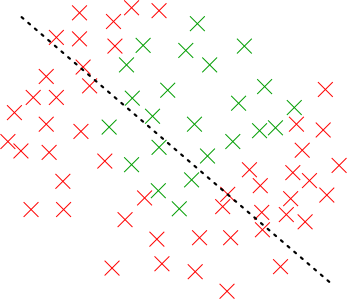
\includegraphics[width=0.3\textwidth]{figures/linsep}
		\caption{Pas de séparation linéaire}
	\end{figure}
\end{frame}

\begin{frame}{Comment ? (2 / 4 maths)}
	\begin{itemize}
		\item Fonction $f: \mathcal{X} \rightarrow \mathbb{R}$
		\item RKHS $\mathcal{H}$ avec évaluation ponctuelle $f(x) = \langle f, K_x \rangle_\mathcal{H}$
		\item Définition noyau:
		\begin{align*}
			k: & (\mathcal{X}, \mathcal{X}) \rightarrow \mathbb{R} \\
			& (x_1, x_2) \mapsto \langle K_{x_1}, K_{x_2}\rangle_\mathcal{H}
		\end{align*}
		\item Application d'un noyau:
		\begin{itemize}
			\item $\mathcal{X} = \mathbf{R}^2$: $k([1, 2], [3, 4]) = -12.2345$
			\item $\mathcal{X} = \text{ChaînesCar}$: $k(\text{toto}, \text{piscine}) = 72.3$
		\end{itemize}
	\end{itemize}
\end{frame}

\begin{frame}{Entracte graphique 1}
	\begin{figure}[b]
		\includegraphics[width=0.7\textwidth]{figures/KernelTrick}
		\caption{$k(x_1, x_2) = \langle x_1, x_2 \rangle + ||x_1||^2 ||x_2||^2$}
	\end{figure}
\end{frame}

\begin{frame}{Entracte graphique 2}
\begin{figure}[b]
	\includegraphics[width=0.7\textwidth]{figures/regression}
	\caption{$k(x_1, x_2)=\exp\left(- \frac{\|\mathbf{x_1} - \mathbf{x_2}\|^2}{2 \sigma^2}\right)$}
\end{figure}
\end{frame}

\begin{frame}{Conclusion de l'entracte}
Complexifier l'espace d'étude, pas l'algorithme.
\end{frame}

\begin{frame}{Génération de caractéristiques (3 / 4 maths)}
\begin{itemize}
	\item Le noyau "crée" les caractéristiques.
	\item Espace de dimension infinie.
\end{itemize}
	\begin{columns}
		\begin{column}{0.45\textwidth}
			\begin{block}{Explicite, manuelle}
				\begin{align*}
				\text{"po po po..."} & \mapsto \begin{bmatrix}
				\text{moy. taille} \\
				\text{n mots} \\
				\vdots \\
				\text{app. dico}
				\end{bmatrix}
				\end{align*}
			\end{block}
		\end{column}
		\begin{column}{0.45\textwidth}
			\begin{block}{Implicite, avec noyaux}
				\begin{align*}
				\text{"po po po..."} & \mapsto \begin{bmatrix}
				12.0 \\
				25.3 \\
				-14.5 \\
				\vdots \\
				\end{bmatrix}
				\end{align*}
			\end{block}
		\end{column}
	\end{columns}
\end{frame}

\begin{frame}{Unification via matrice de Gram (4 / 4 maths)}
	\begin{figure}[t]
		\includegraphics[width=0.8\textwidth]{figures/distance}
	\end{figure}
	
	\begin{table}
		données $\mapsto$
		\begin{tabular}{ |c|c|c|c| }
			\hline
			$k(x_1, x_1)$ & $\cdots$  & $k(x_1, x_n)$ \\
			\hline
			$k(x_2, x_1)$ & $\cdots$ & $k(x_2, x_n)$ \\
			\hline
			$\cdots$ & $\ddots$ & $\cdots$ \\
			\hline
			$k(x_n, x_1)$ & $\cdots$ & $k(x_n, x_n)$ \\
			\hline
		\end{tabular}
	$\mapsto$ algorithmes spécialisés
	\end{table}
\end{frame}

\section{Implémentation}

\begin{frame}{Modularité} %  ne pas détailler, expliquer en quoi la modularité est importante
	\begin{columns}
		\begin{column}{0.3\textwidth}
			\begin{block}{Commun}
				\begin{itemize}
					\item Entrées / Sorties
					\item Matrice de Gram
					\item KerEval
					\item ...
				\end{itemize}
			\end{block}
		\end{column}
		\begin{column}{0.3\textwidth}
			\begin{block}{Données}
				\begin{itemize}
					\item Réels
					\item Vecteurs
					\item Matrices
					\item ...
				\end{itemize}
			\end{block}
			\begin{block}{Noyaux}
				\begin{itemize}
					\item Linéaire
					\item Polynomial
					\item Gaussien
					\item Laplacien
					\item ...
				\end{itemize}
			\end{block}
		\end{column}
		\begin{column}{0.3\textwidth}
			\begin{block}{Algorithmes}
				\begin{itemize}
					\item Régression
					\item Classification non supervisée
					\item Test de distribution
					\item Segmentation
					\item Classification supervisée
					\item ...
				\end{itemize}
			\end{block}
		\end{column}
	\end{columns}
\end{frame}

\begin{frame}{Exemple de données}
\begin{figure}[t]
	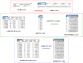
\includegraphics[width=0.8\textwidth]{figures/data}
\end{figure}
\end{frame}

\section{Caractéristiques}

\begin{frame}{Similaire / MixtComp}
	\begin{itemize}
		\item Génération de modèles à partir de briques de base.
		\item Généralisation de codes au coup par coup des chercheurs.
		\item Données complexes sans plongement explicite.
		\item Plus lent mais plus précis que les méthodes de base, type régressions linéaires / logistiques.
	\end{itemize}
\end{frame}

\begin{frame}{Avantages / MixtComp}
	\begin{itemize}
		\item Algorithmes multiples, adaptés à chaque tâche.
		\item Algorithmes non stochastiques, convergence plus rapide, moins de cas limites.
		\item API 1 vs 16 par "modèle".
		\item Pas de modèle par variable $\mapsto$ moins de dégénérescence.
	\end{itemize}
\end{frame}

\begin{frame}{Inconvénients / MixtComp}
	\begin{itemize}
		\item Poids et paramètres de noyau.
		\item Pas de données manquantes (pour le moment).
		\item Algorithmes de base fortement consommateurs en temps et mémoire.
		\item Pas d'outil d'analyse génériques (à voir algo par algo).
	\end{itemize}
\end{frame}

\section{Applications}

\begin{frame}{La vie d'une ville en noyaux}
	\begin{figure}[t]
	\includegraphics[width=0.7\textwidth]{figures/Springfield}
\end{figure}

	\begin{itemize}
		\item Régression: prix d'une maison.
		\item Class.non sup.: groupes de maisons similaires.
		\item Test de dist.: groupes appartiennent à même zone ?
		\item Segmentation: quartier s'embourgeoise ?
		\item Class. supervisée: maison vendue en moins de trois mois ?
	\end{itemize}
\end{frame}

\section{Conclusion}

\begin{frame}{Conclusion}
	\begin{itemize}
		\item Apprentissage / prédiction $\mapsto$ démonstration de faisabilité complète.
		\item À venir: tests sur données réelles et optimisations.
		\item Structures algébriques et programmation fonctionnelles.
		\item Potentiel important / faibles moyens déployés pour le moment.
	\end{itemize}
\end{frame}

\end{document}